\begin{figure*}[t]
\centering
\begin{minipage}[t]{0.49\textwidth}
\centering
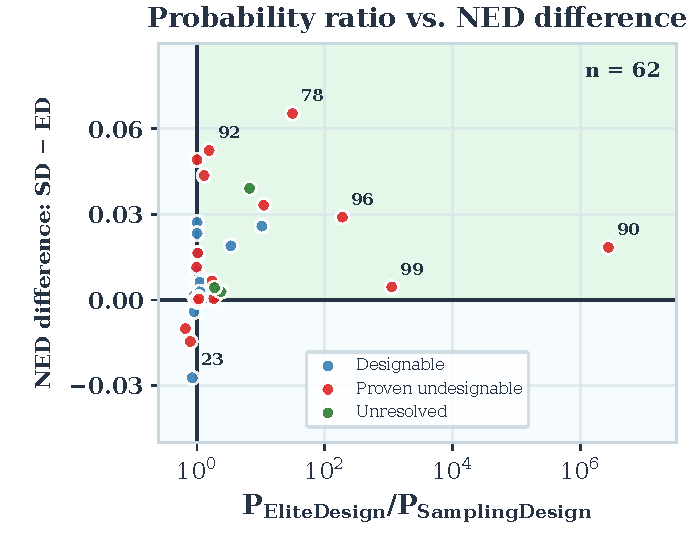
\includegraphics[width=\linewidth]{figures/results/eterna_quadrant_zoom.pdf}
\caption{EliteDesign ($N=500$) versus SamplingDesign on individual Eterna100 puzzles. The $x$-axis is the ratio of their Boltzmann probabilities, and the $y$-axis is SamplingDesign's NED minus EliteDesign's NED. The top right corner shows that EliteDesign is better than SamplingDesign on both metrics for 62 puzzles.}
\label{fig:eterna-advantage}
\end{minipage}\hfill
\begin{minipage}[t]{0.49\textwidth}
\centering
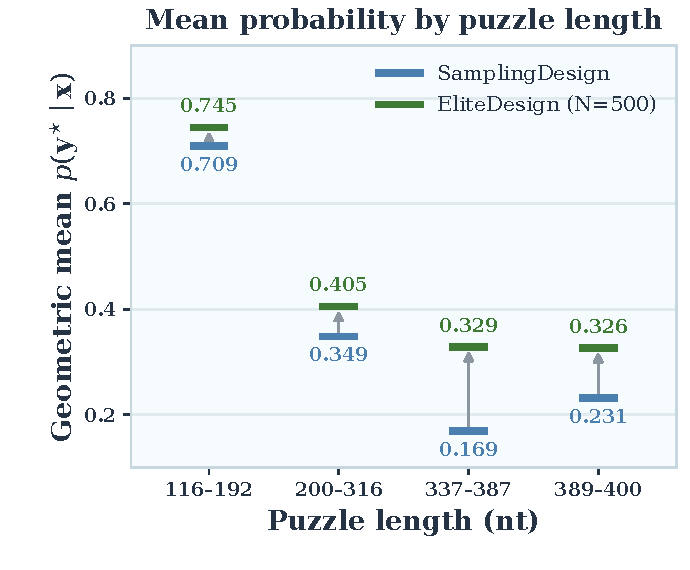
\includegraphics[width=\linewidth]{figures/results/eterna_probability_zoom.pdf}
\caption{Geometric mean Boltzmann probability for the 40 longest Eterna100 puzzles, in four groups of 10 by length. Proven undesignable puzzles are removed from each group, as in SamplingDesign~\citep{tang2026}. The gain from EliteDesign ($N=500$) is largest on long puzzles.}
\label{fig:eterna-length}
\end{minipage}
\end{figure*}
